\section{Software Quality Metrics}
Citat fra Troels: \textit{''Hvad kan man finde ud af om sit program, uden at køre det? Denne disciplin kaldes Static Analysis, og kan give feedback til programmøren, der er ligeså værdifuld som en faktisk test.''}\\

Statisk analyse kan bruges til: 

\begin{enumerate}
	\item Give \textit{quality measures}.
	\item Gennemtvinge \textit{code style and decipline}.
	\item Finde \textit{possible errors}.
\end{enumerate}

Compileren er et eksempel på et Statisk analyseværktøj. Alle moderne compilere viser advarseler og lignende for koden, nogle vigtige, andre not so much.

\subsection{Quantitative code analysis}
Aka: Software Metrics. Bruges til at beskrive: 

\begin{itemize}
	\item Lines of code per function/module.
	\item Cyclomatic complexity (se afsnit~\ref{sec:cyclomatic}).\todo{Sæt dette label på afsnit om cyclomatic complexity.}
	\item Microsoft Maintainability index.
	\item Other measurements.
\end{itemize}

\begin{figure}[H]
\centering
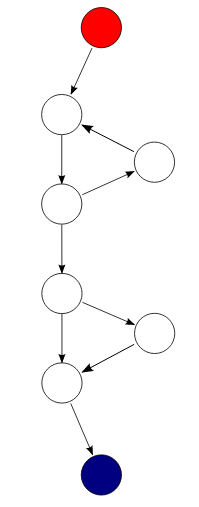
\includegraphics[width=0.25\linewidth]{figs/cyclomatic}
\caption{Grafisk fremstiling af cyclomatisk complexity.}
\label{fig:cyclomatic}
\end{figure}
